\documentclass[12pt]{beamer}

\usepackage[brazil]{babel}
\usepackage[utf8]{inputenc}
\usepackage[T1]{fontenc}
\usepackage{animate}
\usepackage{amsbsy}
\usepackage{amsfonts}
\usepackage{amsmath}
\usepackage{amssymb}
\usepackage{amsthm}
\setbeamertemplate{theorems}[numbered] % to number
\usepackage[toc,page,title,titletoc]{appendix}
\usepackage{dsfont}
\usepackage{esvect}
\usepackage[labelfont=bf]{caption}
%\usepackage{subcaption}
\usepackage{float}
\usepackage[Glenn]{fncychap}%Sonny %Conny %Lenny %Glenn %Renje %Bjarne %Bjornstrup
\usepackage{graphicx}
\usepackage{subfig}
\usepackage{indentfirst}%Para indentar os paragrafos automáticamente
\usepackage{lipsum}
\usepackage{longtable}
\usepackage{mathtools}
\usepackage{listings}%Inserir codigo do R no latex
\usepackage{multirow}
\usepackage{multicol}
\usepackage{csquotes}
\usepackage[maxcitenames=2,terseinits=true,natbib=true, style=authoryear, maxbibnames=99]{biblatex}
\addbibresource{../Referencias/Referencias.bib}
\usepackage[figuresright]{rotating}
\usepackage{spalign}
\usepackage{pgfplots}
\pgfplotsset{compat=1.17}
\usepackage{tikz}
\usepackage{fontawesome}
\usepackage{color, colortbl}
\usepackage{url}
\usepackage{cancel}
\usepackage{accents}
\usepackage{bm}
\usepackage{ragged2e}%para justificar o texto dentro de algum ambiente
\definecolor{Gray}{gray}{0.9}
\definecolor{LightCyan}{rgb}{0.88,1,1}


\usepackage[all]{xy}
\usepackage{hyperref,bookmark}
\hypersetup{
  colorlinks=true,
  linkcolor=blue,
  citecolor=red,
  filecolor=blue,
  urlcolor=blue,
}

\usetheme{Madrid}
\usecolortheme[RGB={193,0,0}]{structure}

%\setbeamertemplate{footline}[frame number]
%\setbeamertemplate{footline}[text line]{%
%  \parbox{\linewidth}{\vspace*{-8pt}\hfill\date{}\hfill\insertshortauthor\hfill\insertpagenumber}}
\beamertemplatenavigationsymbolsempty
\renewcommand{\vec}[1]{\mbox{\boldmath$#1$}}
\newtheorem{Teorema}{Teorema}
\newtheorem{Proposicao}{Proposição}
\newtheorem{definicao}{Definição}
\newtheorem{Corolario}{Corolário}
\newtheorem{Demonstracao}{Demonstração}
\newcommand{\bx}{\ensuremath{\bar{x}}}
\newcommand{\Ho}{\ensuremath{H_{0}}}
\newcommand{\Hi}{\ensuremath{H_{1}}}
\newcommand{\at}[2][]{#1|_{#2}}
\newcommand\xuparrow[1][2ex]{%
   \mathrel{\rotatebox{-90}{$\xleftarrow{\rule{#1}{0pt}}$}}
}
\apptocmd{\frame}{}{\justifying}{} % Allow optional arguments after frame.

\makeatletter
\setbeamertemplate{footline}
{
  \leavevmode%
  \hbox{%
  \begin{beamercolorbox}[wd=.3\paperwidth,ht=2.25ex,dp=1ex,center]{author in head/foot}%
    \usebeamerfont{author in head/foot}\mytext
  \end{beamercolorbox}%
  \begin{beamercolorbox}[wd=.3\paperwidth,ht=2.25ex,dp=1ex,center]{title in head/foot}%
    \usebeamerfont{title in head/foot}\mytextt
  \end{beamercolorbox}%
  \begin{beamercolorbox}[wd=.35\paperwidth,ht=2.25ex,dp=1ex,right]{site in head/foot}%
    \usebeamerfont{site in head/foot}\mytexttt\hspace*{2em}
    \insertframenumber{} / \inserttotalframenumber\hspace*{2ex} 
  \end{beamercolorbox}}%
  \vskip0pt%
}
\makeatother

\providecommand{\arcsin}{} \renewcommand{\arcsin}{\hspace{2pt}\textrm{arcsen}}
\providecommand{\sin}{} \renewcommand{\sin}{\hspace{2pt}\textrm{sen}}
\newcommand{\N}{\rm I\!N}
\newcommand{\I}{\rm I\!I}
\newcommand{\R}{\rm I\!R}
\newcommand{\Sim}{\overset{\text{iid}}{\sim}}
\newcommand{\Lim}{{\displaystyle \lim_{n\to\infty}}}
\newcommand{\LimInf}{{\displaystyle \liminf_{n\to\infty}}}
\newcommand{\rightLim}{\xrightarrow[n\rightarrow\infty]{}}
\newcommand{\Sumi}{{\displaystyle \sum_{i=1}^{n}}}
\newcommand{\Int}{{\displaystyle \int_{-\infty}^{+\infty}}}
\newcommand{\ConvD}{\overset{D}{\rightarrow}}
\newcommand{\ConvP}{\overset{P}{\rightarrow}}
\newcommand{\Prodi}{{\displaystyle \prod_{i=1}^{n}}}
\newcommand{\SetaUP}[2]{\underset{\mathclap{\substack{\xuparrow[30pt] \\ #1}}}{#2}}
%\newcommand{\SetaInclinada}[2]{\underset{\mathclap{\substack{\rotatebox{135}{\xuparrow[30pt] \\ #1}}}}{#2}}
\newcommand{\Home}{\begin{tikzpicture}
\node[scale=2] at (3,4) {\text{Para}~\faHome};
\end{tikzpicture}}
\newcommand{\vecX}{\boldsymbol{X}}
\newcommand{\Implica}[1]{\xRightarrow{#1}}
\newcommand{\SeSe}{\iff}
\newcommand{\EscoreA}{\dfrac{\partial}{\partial\theta}\log{f(x,\theta)}}
\newcommand{\EscoreB}{\dfrac{\partial^{2}}{\partial\theta^{2}}\log{f(x,\theta)}}
\newcommand{\cqd}{\text{cqd}~\blacksquare}
\newcommand{\seqX}{$X_{1},\ldots,X_{n}$}
\newcommand{\seqY}{$Y_{1},\ldots,Y_{n}$}
\newcommand{\tend}[1]{\hbox{\oalign{$\bm{#1}$\crcr\hidewidth$\scriptscriptstyle\bm{\sim}$\hidewidth}}}

%\newtheorem{Teorema}{Teorema}
%\newtheorem{Proposicao}{Proposição}
%\newtheorem{Definicao}{Definição}
%\newtheorem{Corolario}{Corolário}
%\newtheorem{Demonstracao}{Demonstração}

\titlegraphic{\hspace*{8cm}\href{https://fsbmat-ufv.github.io/}{
\includegraphics[width=2cm]{figs/mylogo.png}}
}

%Continuar a numeracao em slides diferentes
\newcounter{saveenumi}
\newcommand{\seti}{\setcounter{saveenumi}{\value{enumi}}}
\newcommand{\conti}{\setcounter{enumi}{\value{saveenumi}}}

\resetcounteronoverlays{saveenumi}

% Layout da pagina
\hypersetup{pdfpagelayout=SinglePage}

%Para o \pause funcionar dentro do ambiente align
\makeatletter
\let\save@measuring@true\measuring@true
\def\measuring@true{%
  \save@measuring@true
  \def\beamer@sortzero##1{\beamer@ifnextcharospec{\beamer@sortzeroread{##1}}{}}%
  \def\beamer@sortzeroread##1<##2>{}%
  \def\beamer@finalnospec{}%
}
\makeatother
\setLayoutColor{2} 

\title{Inferência Estatística II}
\author{Prof. Fernando de Souza Bastos\texorpdfstring{\\ fernando.bastos@ufv.br}{}}
\institute{Departamento de Estatística\texorpdfstring{\\ Programa de Pós-Graduação em Estatística Aplicada e Biometria}\texorpdfstring{\\ Universidade Federal de Viçosa}{}\texorpdfstring{\\ Campus UFV - Viçosa}{}}
\date{}
\newcommand\mytext{Aula 8}
\newcommand\mytextt{Fernando de Souza Bastos}
\newcommand\mytexttt{\url{https://est711.github.io/}}


\begin{document}
%\SweaveOpts{concordance=TRUE}

\frame{\titlepage}

\begin{frame}{}
\frametitle{\bf Sumário}
\tableofcontents
\end{frame}

\section{O Método da Quantidade Pivotal}
\begin{frame}{}
\begin{block}{}
\justifying
\textbf{Definição} Uma variável aleatória $Q(X_1, \ldots, X_n; \theta) = Q(\Vec{X}; \theta)$ é dita ser uma quantidade Pivotal para o parâmetro $\theta$ se sua distribuição for independente de $\theta$.
\end{block}
\end{frame}

\begin{frame}{Exemplo 1}
\begin{block}{}
\justifying
Considere $\Vec{X}=$(\seqX)~ amostra aleatória de $X\sim N(\theta,1),~\theta\in \R.$ Segue que, são quantidades pivotais:
\begin{align*}
     Q_{1}(\Vec{X},\theta)=X_{1}-\theta\sim N(0,1)
\end{align*}
\end{block}
\pause
\begin{block}{}
\justifying
\begin{align*}
    Q_{2}(\Vec{X},\theta)=\dfrac{(\Bar{X}-\theta)}{\sqrt{\frac{1}{n}}}=\sqrt{n}(\Bar{X}-\theta)\sim N(0,1)\\
\end{align*}
\end{block}
\pause
\begin{block}{}
\justifying
\begin{align*}
    Q_{3}(\Vec{X},\theta)=\sqrt{n}\dfrac{(\Bar{X}-\theta)}{S_{n-1}^{2}}\sim t_{n-1}
\end{align*}
\end{block}
\end{frame}

\begin{frame}{Exemplo 2}\label{EX2}
\begin{block}{}
\justifying
Sejam $X_1, \ldots, X_n$ uma amostra aleatória da distribuição da variável aleatória $X$, com densidade

\begin{align}
f(x|\theta) &= \theta e^{-\theta x}, \quad \theta > 0, \; x > 0. \label{eq:densidade}
\end{align}

Como vimos anteriormente, a estatística $T = \Sumi X_i$ é suficiente para $\theta$. Mas, como a distribuição de $T$ é Gama$(n, \theta)$, temos que $T$ não é uma quantidade pivotal para $\theta$. 
\end{block}
\end{frame}

\begin{frame}{}
\begin{block}{}
\justifying
Por outro lado, a densidade de $Q(X;\theta) = 2\theta\Sumi X_i$ é dada por

\begin{align}
f_Q(y) &= \frac{y^{n-1}e^{-y/2}}{2^n\Gamma[n]}, \quad y > 0,
\end{align}

que corresponde à densidade de uma distribuição qui-quadrado com $2n$ graus de liberdade, denotada por $\chi^2_{2n}$. Portanto, $Q(X;\theta)$ pode ser considerada como uma quantidade pivotal, pois sua distribuição é independente de $\theta$. 
\end{block}
\end{frame}

\begin{frame}{Exemplo 3}
\begin{block}{}
\justifying
$\Vec{X}=$(\seqX)~amostra aleatória de $X\sim N(\mu,\sigma^{2})$ em que $\theta=(\mu,\sigma^{2}).$
\begin{align*}
    Q(\mu,\Vec{X})=\sqrt{n}\dfrac{\Bar{X}-\mu}{\sqrt{S^{2}_{n-1}}}\sim t_{(n-1)}~\text{é uma quantidade pivotal para}~\mu\\
     Q(\sigma^{2},\Vec{X})=(n-1)\dfrac{S_{n-1}^{2}}{\sigma^{2}}\sim \chi_{(n-1)}^{2}~\text{é uma quantidade pivotal para}~\sigma^{2}\\
\end{align*}
\end{block}
\end{frame}

\subsection{Quantidade Pivotal Assintótica}
\begin{frame}{Exemplo de Quantidade Pivotal Assintótica}
\begin{block}{}
\justifying
Considere $\Vec{X}=(X_{1},\cdots, X_{n})$ amostra aleatória de $X\sim~$Bernoulli$(\theta),~\theta\in(0,1).$ Notem que $Q(\Vec{X},\theta)=\sqrt{n}\dfrac{(\Bar{X}-\theta)}{\sqrt{\Bar{X}(1-\Bar{X})}}$ é uma quantidade pivotal assintótica, pois, pelo TLC temos que, $$\sqrt{n}(\Bar{X}-\theta)\ConvD N(0,\theta(1-\theta))\Rightarrow~\dfrac{\sqrt{n}(\Bar{X}-\theta)}{\sqrt{\theta(1-\theta)}}\ConvD N(0,1)$$
\end{block}
\end{frame}

\begin{frame}{}
\begin{block}{}
\justifying
Lembrem-se que $\forall \theta\in (0,1)~\Bar{X}\ConvP \theta \Rightarrow \Bar{X}(1-\Bar{X})\ConvP \theta(1-\theta)$
\end{block}
\pause
\begin{block}{}
\justifying
$\Rightarrow~\forall \theta\in (0,1)~\dfrac{\Bar{X}(1-\Bar{X})}{\theta(1-\theta)}\ConvP 1~\Rightarrow\sqrt{\dfrac{\Bar{X}(1-\Bar{X})}{\theta(1-\theta)}}\ConvP 1$
\end{block}
\pause
\begin{block}{}
\justifying
Pelo teorema de Slutsky,
\begin{align*}
\sqrt{n}\dfrac{(\Bar{X}-\theta)}{\sqrt{\cancel{\theta(1-\theta)}}}\dfrac{1}{\sqrt{\dfrac{\Bar{X}(1-\Bar{X})}{\cancel{\theta(1-\theta)}}}}\ConvD N(0,1)
\end{align*}
\end{block}
\end{frame}

\section{Intervalos de Confiança com o Uso de Quantidades Pivotais}
\begin{frame}{Intervalos de Confiança com o Uso de Quantidades Pivotais}
\begin{block}{}
\justifying
Notemos que uma quantidade Pivotal não é uma estatística, pois ela depende de um parâmetro $\theta$ desconhecido. Podemos, então, para cada $\gamma = 1 - \alpha$ fixado, encontrar $\lambda_1$ e $\lambda_2$ na distribuição de $Q(\Vec{X}; \theta)$ de modo que
\begin{align}\label{eq1}
    P[\lambda_1 \leq Q(\Vec{X}; \theta) \leq \lambda_2] = \gamma.
\end{align}
\end{block}
\end{frame}

\begin{frame}{}
\begin{block}{}
\justifying
Sendo a distribuição de $Q(\Vec{X}; \theta)$ independente de $\theta$, $\lambda_1$ e $\lambda_2$ também não dependem de $\theta$. Além disso, se para cada $\Vec{X}$ existirem estatísticas $t_1(\Vec{X})$ e $t_2(\Vec{X})$ tais que
$\lambda_1 \leq Q(\Vec{X}; \theta) \leq \lambda_2$ se e somente se $t_1(\Vec{X}) \leq \theta \leq t_2(\Vec{X})$,
então,
\begin{align}\label{eq2}
    P[t_1(\Vec{X}) \leq \theta \leq t_2(\Vec{X})] = \gamma
\end{align}
de modo que $[t_1(\Vec{X}); t_2(\Vec{X})]$ é um intervalo (aleatório) que contém $\theta$ com probabilidade (coeficiente de confiança) $\gamma = 1 - \alpha$. 
\end{block}
\end{frame}

\begin{frame}{}
\begin{block}{}
\justifying
Nos casos em que a distribuição da variável aleatória $X$ é discreta, em geral, não se consegue determinar $\lambda_1$ e $\lambda_2$ de tal forma que (\ref{eq1}) esteja satisfeita exatamente. Em tais casos, podemos escolher $\lambda_1$ e $\lambda_2$ tal que (\ref{eq1}) esteja satisfeita para um coeficiente de confiança maior ou igual a $\gamma$ (o mais próximo possível).



\end{block}
\end{frame}

\begin{frame}{}
\begin{block}{}
\justifying
Quando $n$ é razoavelmente grande, uma alternativa seria considerar os intervalos de confiança baseados na distribuição do estimador de máxima verossimilhança. Outro ponto a salientar é que, na maioria dos casos, existem muitos pares $(\lambda_1, \lambda_2)$ satisfazendo (\ref{eq1}). Sempre que possível, devemos escolher $(\lambda_1, \lambda_2)$ que produz o intervalo de menor comprimento. Tal procedimento é facilitado em situações em que a distribuição de $Q(\Vec{X}; \theta)$ é simétrica, como no caso da distribuição normal.
\end{block}
\end{frame}

\begin{frame}{Exemplo 1 - Continuação do Exemplo 2 da seção anterior}
\begin{block}{}
\justifying
No Exemplo 2 da página\hyperlink{EX2}{ \pageref{EX2}} dado o coeficiente de confiança $\gamma = 1 - \alpha$, obtemos $\lambda_1$ e $\lambda_2$ na tabela da distribuição $\chi^2_{2n}$, de modo que

\begin{align}\label{eq5}
P\left(\lambda_1 \leq 2\theta\sum_{i=1}^{n} X_i \leq \lambda_2\right) = \gamma,
\end{align}
\end{block}
\end{frame}

\begin{frame}{}
\begin{block}{}
\justifying
Logo, um intervalo de confiança para $\theta$ com coeficiente de confiança $\gamma$ é dado por

\begin{align}\label{I6}
\left[ \frac{\lambda_1}{2\Sumi X_i} ; \frac{\lambda_2}{2\Sumi X_i} \right].
\end{align}
\end{block}
\end{frame}

\begin{frame}{}
\begin{block}{}
\justifying
existem infinitos pares $(\lambda_1, \lambda_2)$ para os quais (\ref{eq5}) está verificada. Sempre que possível, $(\lambda_1, \lambda_2)$ devem ser escolhidos de modo que o intervalo (\ref{I6}) seja de comprimento mínimo. Tal intervalo existe, mas $(\lambda_1, \lambda_2)$ deve ser obtido por métodos computacionais. Uma alternativa é considerarmos intervalos simétricos em que $(\lambda_1, \lambda_2)$ são obtidos a partir da distribuição $\chi^2_{2n}$, de modo que a área à esquerda de $\lambda_1$ seja igual à área à direita de $\lambda_2$ e igual a $\alpha/2$.
\end{block}
\begin{figure}
    \centering
    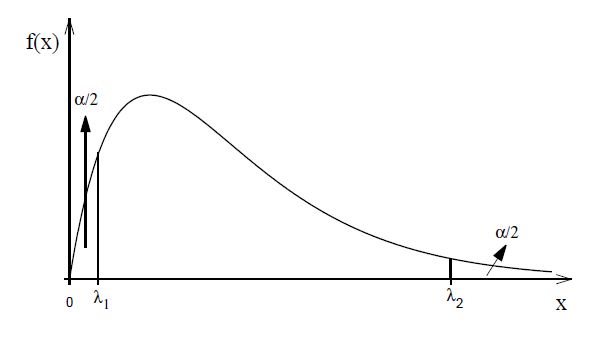
\includegraphics[scale=0.6]{figs/ChiQuad.PNG}
    \label{fig:enter-label}
\end{figure}
\end{frame}

\begin{frame}{Exemplo 2}
\begin{block}{}
\justifying
Seja $\Vec{X}=$\seqX~ amostra aleatória de $X\sim N(\theta,1), \theta\in \R.$
\begin{align*}
    Q(\Vec{X};\theta)=\sqrt{n}\dfrac{(\Bar{X}-\theta)}{\sqrt{S_{n-1}^{2}}}\sim t_{(n-1)}
\end{align*}
\end{block}
\pause
\begin{block}{}
\justifying
\begin{figure}[H]
\centering
\begin{tikzpicture}[line cap=round,line join=round,x=1.9cm,y=4*1.9cm,scale=0.8]
\draw[->,color=black,line width=1.0pt] (-3.5,-0.01) -- (3.7,-0.01);
\draw (3.8,-0.01) node[] {$\R$};
\draw[shift={(0,0)},color=black,line width=1.0pt] (0,0.02) -- (0,-0.02) node[below] {$0$};
\draw[smooth,samples=100,domain=-3.5:3.5,line width=1.0pt] plot(\x,{(1/sqrt(2*pi))*exp((-(\x)^2)/2)});
\draw[fill=black,fill opacity=0.3, smooth,samples=50,domain=-3.5:-1.5] plot(\x,{(1/sqrt(2*pi))*exp((-(\x)^2)/2)}) -- (-1.5,0) -- (-3.5,0) -- cycle;
\draw [dash pattern=on 3pt off 3pt,line width=1.0pt] (-1.5,0) -- (-1.5,0.3989);
%\draw (-2.5,0.2393) node[right] {$RRH_0$};
\draw [->] (-1.9,0.0399) -- (-2.2,0.1197);
\draw (-2.5,0.2) node[left] {$\dfrac{1-\gamma}{2}$};
\draw (-1.5,0) node[below] {$\lambda_{1}$};
\draw[fill=black,fill opacity=0.3, smooth,samples=50,domain=1.5:3.5] plot(\x,{(1/sqrt(2*pi))*exp((-(\x)^2)/2)}) -- (3.5,0) -- (1.5,0) -- cycle;
\draw [dash pattern=on 3pt off 3pt,line width=1.0pt] (1.5,0) -- (1.5,0.3989);
%\draw (1.6,0.2393) node[right] {$RRH_0$};
%\draw (-0.0,0.2393) node[] {$RNRH_0$};
\draw [->] (1.9,0.0399) -- (2.2,0.1197);
\draw (3,0.2) node[left] {$\dfrac{1-\gamma}{2}$};
\draw (1.5,0) node[below] {$\lambda_{2}$};
\end{tikzpicture}
%\vspace{-.6cm}
%\caption{Região crítica para o teste $Z$, para uma média, bilateral.}\label{Fig:THZRCBil}
\end{figure}
\end{block}
\end{frame}

\begin{frame}{}
\begin{block}{}
\justifying
Notem que
\begin{align*}
    \lambda_{1}\leq \sqrt{n}\dfrac{(\Bar{X}-\theta)}{\sqrt{S_{n-1}^{2}}}\leq \lambda_{2}\SeSe
    \Bar{X}-\lambda_{2}\sqrt{\frac{S_{n-1}^{2}}{n}}\leq \theta \leq \Bar{X}+\lambda_{1}\sqrt{\frac{S_{n-1}^{2}}{n}}
\end{align*}
\end{block}
\pause
\begin{block}{}
\justifying
$$\Rightarrow IC(\theta,\gamma)=\left(\Bar{X}-\lambda_{2}\sqrt{\frac{S_{n-1}^{2}}{n}},\Bar{X}+\lambda_{1}\sqrt{\frac{S_{n-1}^{2}}{n}}\right)$$
\end{block}
\pause
\begin{block}{}
\justifying
Note que este é um intervalo de confiança exato! Basta encontrar $\lambda_{1}$ e $\lambda_{2}$ a partir da distribuição $t$ com $n-1$ graus de liberdade.
\end{block}
\end{frame}

\begin{frame}{}

\begin{block}{}
\justifying
Considere \(\Vec{X}=(X_{1},\cdots,X_{n})\) amostra aleatória de $X\sim~$Bernoulli$(\theta),~\theta\in(0,1).$ Mostramos anteriormente que $Q(\Vec{X},\theta)=\sqrt{n}\dfrac{(\Bar{X}-\theta)}{\sqrt{\Bar{X}(1-\Bar{X})}}\ConvD N(0,1), \forall \theta \in (0,1),$ logo 
\end{block}
\pause
\begin{block}{}
\justifying
\begin{align*}
    \Bar{X}-\lambda_{2}\sqrt{\dfrac{\Bar{X}(1-\Bar{X})}{n}}\leq \theta \leq \Bar{X}+\lambda_{1}\sqrt{\dfrac{\Bar{X}(1-\Bar{X})}{n}}\\
    \Rightarrow IC(\theta,\gamma)=\left(\Bar{X}-\lambda_{1}\sqrt{\dfrac{\Bar{X}(1-\Bar{X})}{n}},\Bar{X}+\lambda_{1}\sqrt{\dfrac{\Bar{X}(1-\Bar{X})}{n}}\right)\cap[0,1],
\end{align*}
em que $\lambda_{1}=-\lambda_{2},~\forall\gamma\in[0,1]$
\end{block}
\pause
\begin{block}{}
\justifying
Nesse caso temos um intervalo de confiança aproximado, pois $\Bar{X}\ConvP \theta.$
\end{block}
\end{frame}

\begin{frame}{Exemplo 3}
\begin{block}{}
\justifying
Sejam $X_1, \ldots, X_n$ uma amostra aleatória de tamanho $n$ da distribuição $N(\mu, \sigma^2)$. Assumindo $\sigma^2$ conhecido, temos que uma quantidade pivotal para $\mu$, baseada na estatística suficiente

\begin{align*}
\frac{1}{n} \sum_{i=1}^{n} X_i = \bar{X},
\end{align*}

é dada por

\begin{align*}
Q(X; \mu) = \frac{\bar{X} - \mu}{\sigma/\sqrt{n}},
\end{align*}

que tem distribuição $N(0, 1)$.
\end{block}
\end{frame}

\begin{frame}{}
\begin{block}{}
\justifying
Por outro lado, sendo $\sigma^2$ desconhecido, temos que

\begin{align*}
Q(X, \mu) = \frac{\bar{X} - \mu}{S/\sqrt{n}} \sim t_{n-1},
\end{align*}

que, nesse caso, é uma quantidade pivotal. Então, dado $\gamma$, existem $\lambda_1$ e $\lambda_2$ na distribuição $t_{n-1}$ de modo que

\begin{align*}
P\left(\lambda_1 \leq \frac{\bar{X} - \mu}{S/\sqrt{n}} \leq \lambda_2\right) = \gamma.
\end{align*}
\end{block}
\end{frame}

\begin{frame}{}
\begin{block}{}
\justifying
Quanto a $\sigma^2$, considerando $\mu$ desconhecido, temos que

\begin{align*}
Q(X, \sigma^2) = \frac{(n - 1)S^2}{\sigma^2} \sim \chi^2_{n-1}
\end{align*}

é uma quantidade pivotal para $\sigma^2$. Portanto, dado $\gamma$, podemos determinar $\lambda_1$ e $\lambda_2$ de modo que

\begin{align*}
P\left(\lambda_1 \leq \frac{(n - 1)S^2}{\sigma^2} \leq \lambda_2\right) = \gamma.
\end{align*}

Considerando o intervalo simétrico, ou seja, $\lambda_1 = q_1$ e $\lambda_2 = q_2$, em que $P[\chi^2_{n-1} \geq q_2] = P[\chi^2_{n-1} \leq q_1] = \alpha/2$, temos o intervalo:

\begin{align*}
\left(\frac{(n - 1)S^2}{q_2}; \frac{(n - 1)S^2}{q_1}\right).
\end{align*}
\end{block}
\end{frame}

\section{Intervalos de Confiança Aproximados}
\begin{frame}{Intervalos de Confiança Aproximados}
\begin{block}{}
\justifying
Já vimos que, se $\hat{\theta}$ é o EMV de $\theta,$ então 
\begin{align*}
    \dfrac{\hat{\theta}-\theta}{\sqrt{(nI(\theta))^{-1}}}\ConvD N(0,1)
\end{align*}
\end{block}
\pause
\begin{block}{}
\justifying
Como $I(\theta)$ pode depender de $\theta$, que não é conhecido, substituindo $I(\theta)$ por $I(\hat{\theta})$, temos que

\begin{align*}
Q(X, \theta) = \frac{\hat{\theta} - \theta}{\sqrt{(nI(\hat{\theta}))^{-1}}} \sim N(0, 1),
\end{align*}

de modo que $Q(X, \theta)$ é uma quantidade pivotal com distribuição aproximadamente igual à distribuição $N(0, 1)$ em grandes amostras.
\end{block}
\end{frame}

\begin{frame}{}
\begin{block}{}
\justifying
Com relação a uma função $g(\theta)$, podemos considerar a variável aleatória

\begin{align*}
Q(X, g(\theta)) = \frac{g(\hat{\theta}) - g(\theta)}{\sqrt{\dfrac{(g'(\hat{\theta}))^2}{nI(\hat{\theta})}}} \sim N(0, 1),
\end{align*}
que, para amostras grandes, é uma quantidade pivotal.
\end{block}
\end{frame}

\begin{frame}{Exemplo 1}
\begin{block}{}
\justifying
Sejam $X_1, \ldots, X_n$ uma amostra aleatória da variável aleatória $X \sim \text{Bernoulli}(\theta)$. Como o estimador de máxima verossimilhança de $\theta$ é $\hat{\theta} = \Bar{X}$ e $I(\theta) = \frac{1}{\theta(1 - \theta)}$, temos que uma quantidade pivotal para $\theta$ é dada por
\begin{align*}
Q(X, \theta) = \frac{\bar{X} - \theta}{\sqrt{\frac{\bar{X}(1-\bar{X})}{n}}} \sim N(0, 1),
\end{align*}
de modo que para valores grandes de $n$, um intervalo de confiança para $\theta$ com coeficiente de confiança aproximadamente $\gamma$ é dado por
\begin{align*}
\left[ \bar{X} - z_{\frac{\alpha}{2}} \sqrt{\frac{\bar{X}(1 - \bar{X})}{n}} ; \bar{X} + z_{\frac{\alpha}{2}} \sqrt{\frac{\bar{X}(1 - \bar{X})}{n}} \right].
\end{align*}
\end{block}
\end{frame}

\begin{frame}{}
\begin{block}{}
\justifying
Suponhamos agora que seja de interesse a obtenção de um intervalo de confiança para $g(\theta) = \theta(1 - \theta)$. Como $g'(\theta) = 1 - 2\theta$ e $I(\theta) = \frac{1}{\theta(1 - \theta)}$, temos que uma quantidade pivotal para $g(\theta)$ é dada por

\begin{align*}
Q(X, \theta) = \dfrac{\hat{\theta}(1 - \hat{\theta}) - \theta(1 - \theta)}{\sqrt{\dfrac{\hat{\theta}(1-\hat{\theta})(1-2\hat{\theta})^2}{n}}} \sim N(0, 1),
\end{align*}

de modo que um intervalo de confiança aproximado para $g(\theta) = \theta(1-\theta)$ é dado por

{\footnotesize
\begin{align*}
\left[ \bar{X}(1 - \bar{X}) - z_{\frac{\alpha}{2}} \sqrt{\frac{\bar{X}(1 - \bar{X})(1 - 2\bar{X})^2}{n}} ; \bar{X}(1 - \bar{X}) + z_{\frac{\alpha}{2}} \sqrt{\frac{\bar{X}(1 - \bar{X})(1 - 2\bar{X})^2}{n}} \right],
\end{align*}
}

em que $z_{\frac{\alpha}{2}}$ é obtido na tabela da distribuição $N(0, 1)$.
\end{block}
\end{frame}

\begin{frame}{Exemplo 2}
\begin{block}{}
\justifying
Sejam $X_1, \ldots, X_n$ uma amostra aleatória de tamanho $n$ da variável aleatória $X \sim \text{Exp}(\theta)$, com função densidade

\begin{align*}
f(x|\theta) = \theta e^{-\theta x}, \quad x > 0, \; \theta > 0.
\end{align*}

Como $I^{-1}(\theta) = \theta^2$ e $\hat{\theta} = \dfrac{1}{\Bar{X}}$, segue que uma quantidade pivotal para $\theta$ é dada por

\begin{align*}
Q(X, \theta) = \dfrac{\dfrac{1}{\Bar{X}} - \theta}{\sqrt{\dfrac{\hat{\theta}^2}{n}}} \sim N(0, 1),
\end{align*}

\end{block}
\end{frame}

\begin{frame}{}
\begin{block}{}
\justifying
de modo que um intervalo de confiança com coeficiente de confiança aproximado $\gamma = 1 - \alpha$ é dado por

\begin{align*}
\left( \dfrac{1}{\Bar{X}} - z_{\dfrac{\alpha}{2}} \sqrt{\dfrac{1}{n\Bar{X}^2}} ; \dfrac{1}{\Bar{X}} + z_{\dfrac{\alpha}{2}} \sqrt{\dfrac{1}{n\Bar{X}^2}} \right).
\end{align*}
\end{block}
\nocite{bolfarine}
\end{frame}

%\begin{frame}{\Home}
%\begin{block}{}
%\justifying

%\begin{itemize}
%    \item \textbf{Exercícios da seção 4.2:} 25 ao 27.
%\end{itemize}

%\end{block}
%\end{frame}

\begin{frame}[allowframebreaks]
\frametitle{\bf Referências}
\printbibliography
\end{frame}


\end{document}
